\documentclass[aspectratio=169]{beamer}

\input{preamble.tex}

\title[Galois Distributed --- масштабируемость]{Распределённая обработка графов:\\исследование масштабируемости Galois Distributed}
\institute[СПбГУ]{}
\author[Гавриленко Михаил]{Гавриленко Михаил, группа 23.Б15-мм}

\begin{document}

% ── Титульный лист ────────────────────────────────────────────────────────────
{
\setbeamertemplate{footline}{}
\begin{frame}
  
\includegraphics[width=1.4cm]{pictures/SPbGU_Logo.png}
  \vspace{-35pt}
  \hspace{-10pt}
  \begin{center}
    \begin{tabular}{c}
      \scriptsize{Санкт-Петербургский государственный университет} \\
      \scriptsize{Кафедра системного программирования}
    \end{tabular}
    \titlepage
  \end{center}
  \btVFill
  \begin{center}
    \vspace{5pt}
    \scriptsize{Санкт-Петербург\\ 2025}
  \end{center}
\end{frame}
}

% ── Постановка задачи ─────────────────────────────────────────────────────────
\begin{frame}
  \frametitle{Постановка задачи}

  \textbf{Цель:} исследовать сильное масштабирование BFS, PageRank и SSSP
  при увеличении числа MPI-процессов в Galois Distributed.

  \textbf{Задачи:}
  \begin{itemize}
    \item Сформулировать и проверить гипотезы о масштабируемости
    \item Провести эксперименты: $P \in \{1,2,4,6,8\}$ MPI-процессов
          на 3 структурно разных графах, $T=2$ OpenMP-потока (фиксировано)
  \end{itemize}
\end{frame}

% ── Платформа ─────────────────────────────────────────────────────────────────
\begin{frame}
  \frametitle{Платформа: Galois Distributed + Gluon}

  \textbf{Модель BSP} (Bulk-Synchronous Parallel):
  \[
    \underbrace{\text{Compute}}_{\text{локальные вычисления}}
    \;\to\;
    \underbrace{\text{Communicate}}_{\text{Gluon sync}}
    \;\to\;
    \underbrace{\text{Barrier}}_{\text{глобальный барьер}}
  \]

  \textbf{Разбиение OEC} (Outgoing Edge-Cut): вершина $v$ и все её
  исходящие рёбра $v \to u_i$ на одном процессе.
  Если $u_i$ на другом процессе --- там создаётся \emph{зеркало} $\tilde{u}_i$.

  \medskip
  \textbf{Коэффициент репликации} RF $=$ среднее число копий вершины:

  \begin{center}
  \small
  \begin{tabular}{lccc}
    \hline
    Граф & RF при $P=2$ & RF при $P=4$ & RF при $P=8$ \\
    \hline
    LiveJournal    & 1.62 & 2.47 & \textbf{3.49} \\
    RGG ($2^{20}$) & 1.000 & 1.001 & 1.002 \\
    RoadNet-PA     & 1.007 & 1.009 & 1.016 \\
    \hline
  \end{tabular}
  \end{center}
\end{frame}

% ── Наборы данных ─────────────────────────────────────────────────────────────
\begin{frame}
  \frametitle{Наборы данных}

  \begin{center}
  \small
  \begin{tabular}{lrrrll}
    \hline
    Граф & Вершин & Рёбер & Ср.\ степень & Диаметр & Тип \\
    \hline
    soc-LiveJournal1  & 4.8М & 69М  & 14.2 & $\approx$5    & Социальный \\
    rgg\_n\_2\_20\_s0 & 1.0М & 7.3М & 7.0  & $\approx$1200 & Геометрический \\
    roadNet-PA        & 1.1М & 3.1М & 1.4  & $\approx$320  & Дорожный \\
    \hline
  \end{tabular}
  \end{center}

  \medskip
  \begin{itemize}
    \item \textbf{LiveJournal} --- RF растёт с $P$;
          малый диаметр $\approx 5$
    \item \textbf{RGG} --- RF\,$\approx 1$ при любом $P$,
          но высокий диаметр $\approx 1200$
    \item \textbf{RoadNet-PA} --- планарный, малая степень, диаметр $\approx 320$
  \end{itemize}
\end{frame}

% ── Методология ───────────────────────────────────────────────────────────────
\begin{frame}
  \frametitle{Методология}
  \textbf{Аппаратура:}
  \begin{itemize}
	\item Apple M2 Max, 12 ядер, macOS Tahoe
	\item MPICH 4.3.0
	\item clang 21.0.0
	\item $T = 2$ OpenMP-потока на процесс (фиксировано)
	\item $P \in \{1, 2, 4, 6, 8\}$
	\item 10 прогонов; run~0 --- прогрев, отброшен
  \end{itemize}

  \medskip
  \textbf{Метрики:}
  \begin{itemize}
	\item $T(P)$ --- время run~1 (мс)
	\item $T(P)/T(1)$ --- нормализованное время\\
		  {\small $< 1$ = быстрее, $> 1$ = медленнее}
	\item $E(P) = \dfrac{T(1)}{P \cdot T(P)}$ --- эффективность
  \end{itemize}
\end{frame}

% ──────────────────────────────────────────────────────────────────────────────
%  BFS
% ──────────────────────────────────────────────────────────────────────────────

\begin{frame}
  \frametitle{BFS --- алгоритм и ключевой код}

  \textbf{Pull-BFS:} каждая вершина $v$ проверяет своих соседей;
  если $\mathrm{dist}(u)+1 < \mathrm{dist}(v)$ --- обновить.
  Один BSP-раунд = один уровень обхода.

  \medskip
  {\small Ключевой оператор (\texttt{bfs\_pull.cpp}):}
  \begin{exampleblock}{}
  \vspace{-4pt}
  {\scriptsize\tt
  \hspace{1em}void operator()(GNode src) \{\\
  \hspace{2em}auto\& snode = graph->getData(src);\\
  \hspace{2em}for (auto jj : graph->edges(src)) \{\\
  \hspace{3em}GNode dst = graph->getEdgeDst(jj);\\
  \hspace{3em}uint32\_t new\_dist = graph->getData(dst).dist\_current + 1;\\
  \hspace{3em}if (galois::min(snode.dist\_current, new\_dist) > new\_dist)\\
  \hspace{4em}bitset\_dist\_current.set(src);\\
  \hspace{2em}\}\\
  \hspace{1em}\}
  }
  \vspace{-4pt}
  \end{exampleblock}

  После каждой итерации Gluon рассылает обновлённые значения по зеркалам:

  {\scriptsize\tt
  syncSubstrate->sync<writeSource, readDestination,
    Reduce\_min\_dist\_current, Bitset\_dist\_current>("BFS");
  }
\end{frame}

\begin{frame}
  \frametitle{BFS --- первичные тезисы}

  \begin{itemize}
    \item \textbf{BFS/LiveJournal:} диаметр $\approx 5$ ---
          мало BSP-раундов; основной overhead --- RF.
          Ожидаем небольшое ускорение, затем деградацию.

    \item \textbf{BFS/RoadNet:} $\sim 320$ BSP-раундов $\times$ стоимость барьера.
          Ожидаем монотонную деградацию.

    \item \textbf{BFS/RGG:}
          диаметр $\approx 1200$. Сильный оверхед на коммуникацию из-за кол-ва операций.
  \end{itemize}
\end{frame}

\begin{frame}
  \frametitle{BFS --- время выполнения ($T=2$, фиксировано)}
  \centering
  
\includegraphics[width=0.5\textwidth]{../results/block2_t2/plots/time_bfs.png}
\end{frame}

\begin{frame}
  \frametitle{BFS --- нормализованное время $T(P)/T(1)$}
  \centering
  
\includegraphics[width=0.5\textwidth]{../results/block2_t2/plots/speedup_bfs.png}

  \smallskip
  {\small $< 1$ --- ускорение; $> 1$ --- деградация. Пунктир --- идеал $1/P$.}
\end{frame}

\begin{frame}
  \frametitle{BFS --- число итераций и время}

  \begin{center}
  {\small
  \begin{tabular}{lrrrrr}
    \hline
    & $P=1$ & $P=2$ & $P=4$ & $P=6$ & $P=8$ \\
    \hline
    BFS/LJ итер.         & 2    & 2    & 4    & 5    & 5    \\
    BFS/LJ $T(P)/T(1)$   & 1.00 & \textbf{0.77} & 1.23 & 2.55 & 3.89 \\
    \hline
    BFS/RGG итер.        & 495  & 929  & 1226 & 2377 & ---  \\
    BFS/RGG время (мс)   & 1557 & 4202 & 14836 & 45067 & timeout \\
    \hline
    BFS/Road итер.       & 318  & 328  & 345  & 379  & 447  \\
    BFS/Road $T(P)/T(1)$ & 1.00 & 0.79 & 2.78 & 6.69 & 11.11 \\
    \hline
  \end{tabular}
  }
  \end{center}

  \begin{itemize}
    \item BFS/LJ при $P{=}2$: 2 итерации, параллелизм помогает --- $T(2)/T(1)=0.77$
    \item BFS/RGG: итерации растут в \textbf{5$\times$} ($P{=}1\to6$) из-за
          staleness --- суперлинейная деградация
  \end{itemize}
\end{frame}

\begin{frame}
  \frametitle{BFS: Push vs Pull на LiveJournal}

  \textbf{Push-BFS:} активная вершина рассылает обновление соседям.\\
  \textbf{Pull-BFS:} вершина проверяет всех своих соседей сама.

  \begin{center}
  {\small
  \begin{tabular}{lrrrrr}
    \hline
    & $P=1$ & $P=2$ & $P=4$ & $P=6$ & $P=8$ \\
    \hline
    Pull (мс) & 53  & 41  & 65  & 135 & 206 \\
    Push (мс) & \textbf{1}   & \textbf{4}   & \textbf{24}  & 113 & 356 \\
    \hline
  \end{tabular}
  }
  \end{center}

  \begin{itemize}
    \item \textbf{Push в 50$\times$ быстрее при $P{=}1$:}
          LJ имеет диаметр $\approx 5$, фронтир мал ---
          Push обрабатывает только активные вершины,
          Pull всегда сканирует все 69М рёбер

    \item \textbf{При $P{=}8$ Push медленнее Pull} ($356$ vs $206$ мс):
          с OEC-разбиением исходящие рёбра активных вершин
          пересекают границы разделов -- больше коммуникации
  \end{itemize}
\end{frame}

% ──────────────────────────────────────────────────────────────────────────────
%  PageRank
% ──────────────────────────────────────────────────────────────────────────────

\begin{frame}
  \frametitle{PageRank}

  \textbf{Гипотезы:}
  \begin{itemize}
    \item PR/LJ: ускорение при $P{=}2$ (высокое Work/Comm),
          деградация при $P{\ge}4$ (RF$+$итерации)
    \item PR/RGG, RoadNet: RF\,$\approx 1$, но итерации растут с $P$
  \end{itemize}
\end{frame}


\begin{frame}
  \frametitle{PageRank --- число итераций}

  \begin{center}
  {\small
  \begin{tabular}{lrrrrr}
    \hline
    & $P=1$ & $P=2$ & $P=4$ & $P=6$ & $P=8$ \\
    \hline
    PR/LJ время (мс)     & 7326 & 5760 & 7710 & 22772 & 26121 \\
    PR/LJ $T(P)/T(1)$    & 1.00 & \textbf{0.79} & 1.05 & 3.11 & 3.57 \\
    PR/LJ итераций       & 93   & 143  & 160  & 424   & 410  \\
    \hline
    PR/RGG $T(P)/T(1)$   & 1.00 & 1.35 & 3.63 & 11.65 & 20.55 \\
    PR/RGG итераций      & 51   & 76   & 74   & 189   & 268  \\
    \hline
    PR/Road $T(P)/T(1)$  & 1.00 & 0.95 & 2.65 & 8.26  & 14.60 \\
    PR/Road итераций     & 51   & 57   & 64   & 99    & 160  \\
    \hline
  \end{tabular}
  }
  \end{center}
\end{frame}

\begin{frame}
  \frametitle{PageRank --- время выполнения}
  \centering
  
\includegraphics[width=0.5\textwidth]{../results/block2_t2/plots/time_pagerank.png}
\end{frame}

\begin{frame}
  \frametitle{PageRank --- нормализованное время $T(P)/T(1)$}
  \centering
  
\includegraphics[width=0.5\textwidth]{../results/block2_t2/plots/speedup_pagerank.png}
\end{frame}

% ──────────────────────────────────────────────────────────────────────────────
%  SSSP
% ──────────────────────────────────────────────────────────────────────────────

\begin{frame}
  \frametitle{SSSP --- результаты}

  \begin{center}
  {\small
  \begin{tabular}{lrrrrr}
    \hline
    & $P=1$ & $P=2$ & $P=4$ & $P=6$ & $P=8$ \\
    \hline
    SSSP/LJ $T(P)/T(1)$   & 1.00 & \textbf{0.79} & 1.00 & 1.61 & 1.85 \\
    SSSP/LJ итераций      & 1    & 1    & 1    & 1    & 1    \\
    \hline
    SSSP/RGG время (мс)   & 3868 & 6618 & 19084 & 41781 & timeout \\
    SSSP/RGG итераций     & 878  & 1000$^*$ & 1000$^*$ & 1000$^*$ & --- \\
    \hline
    SSSP/Road $T(P)/T(1)$ & 1.00 & 0.83 & 2.57 & 10.46 & 28.07 \\
    SSSP/Road итераций    & 375  & 377  & 375  & 374   & 377  \\
    \hline
  \end{tabular}
  }
  \end{center}

  {\small $^*$ --- достигнут лимит \texttt{maxIterations=1000}, алгоритм не сошёлся}

  \begin{itemize}
    \item SSSP/LJ: 1 итерация при любом $P$ --- power-law граф,
          короткие пути $\Rightarrow$ сходится за один проход
    \item SSSP/RGG: не сходится за 1000 раундов при $P{\ge}2$
          (огромный диаметр)
  \end{itemize}
\end{frame}

\begin{frame}
  \frametitle{SSSP --- время выполнения}
  \centering
  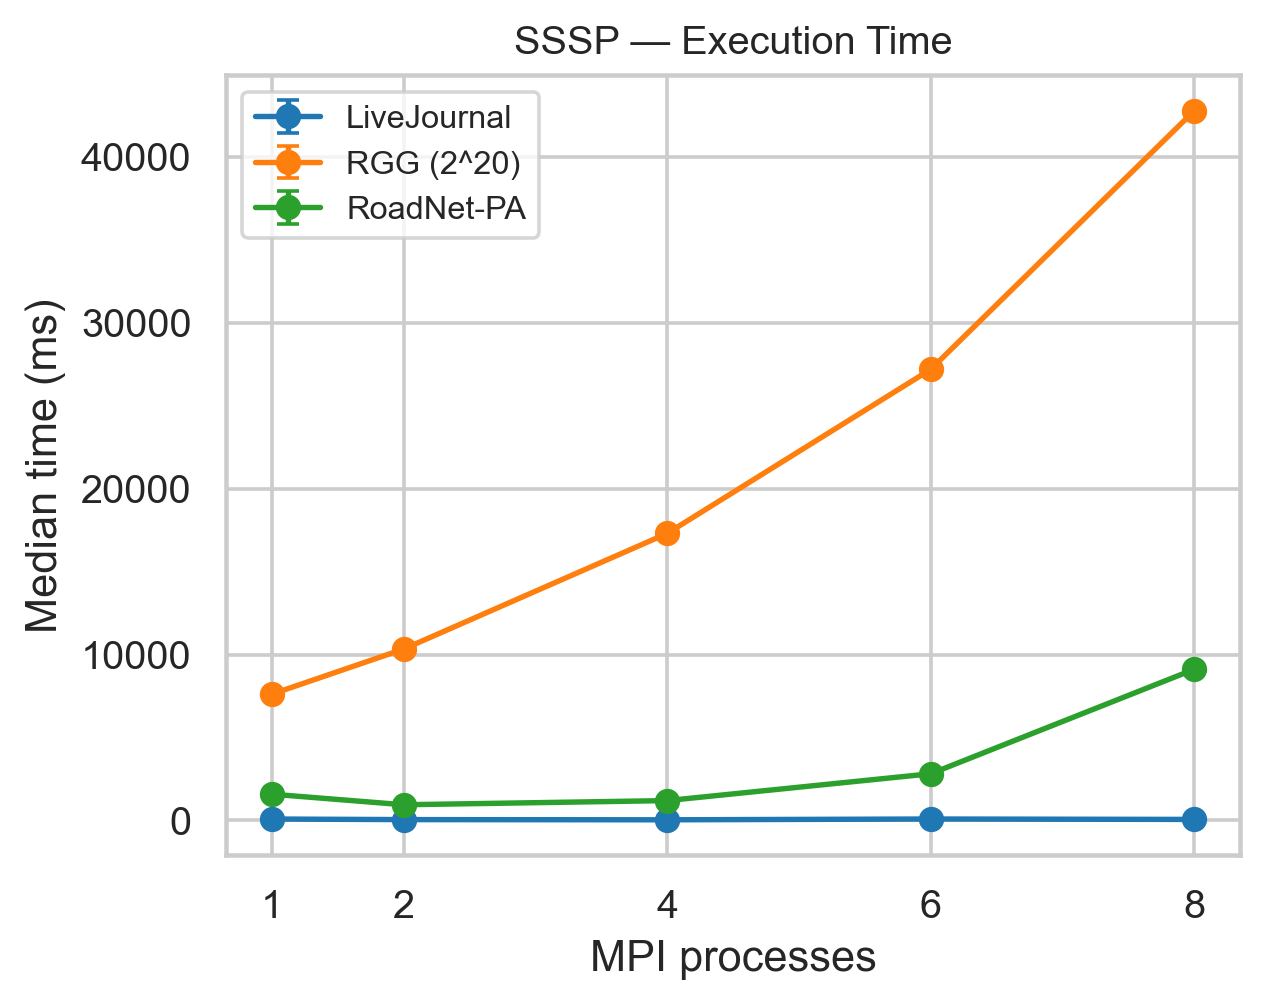
\includegraphics[width=0.5\textwidth]{../results/block2_t2/plots/time_sssp.png}
\end{frame}

\begin{frame}
  \frametitle{SSSP --- нормализованное время $T(P)/T(1)$}
  \centering
  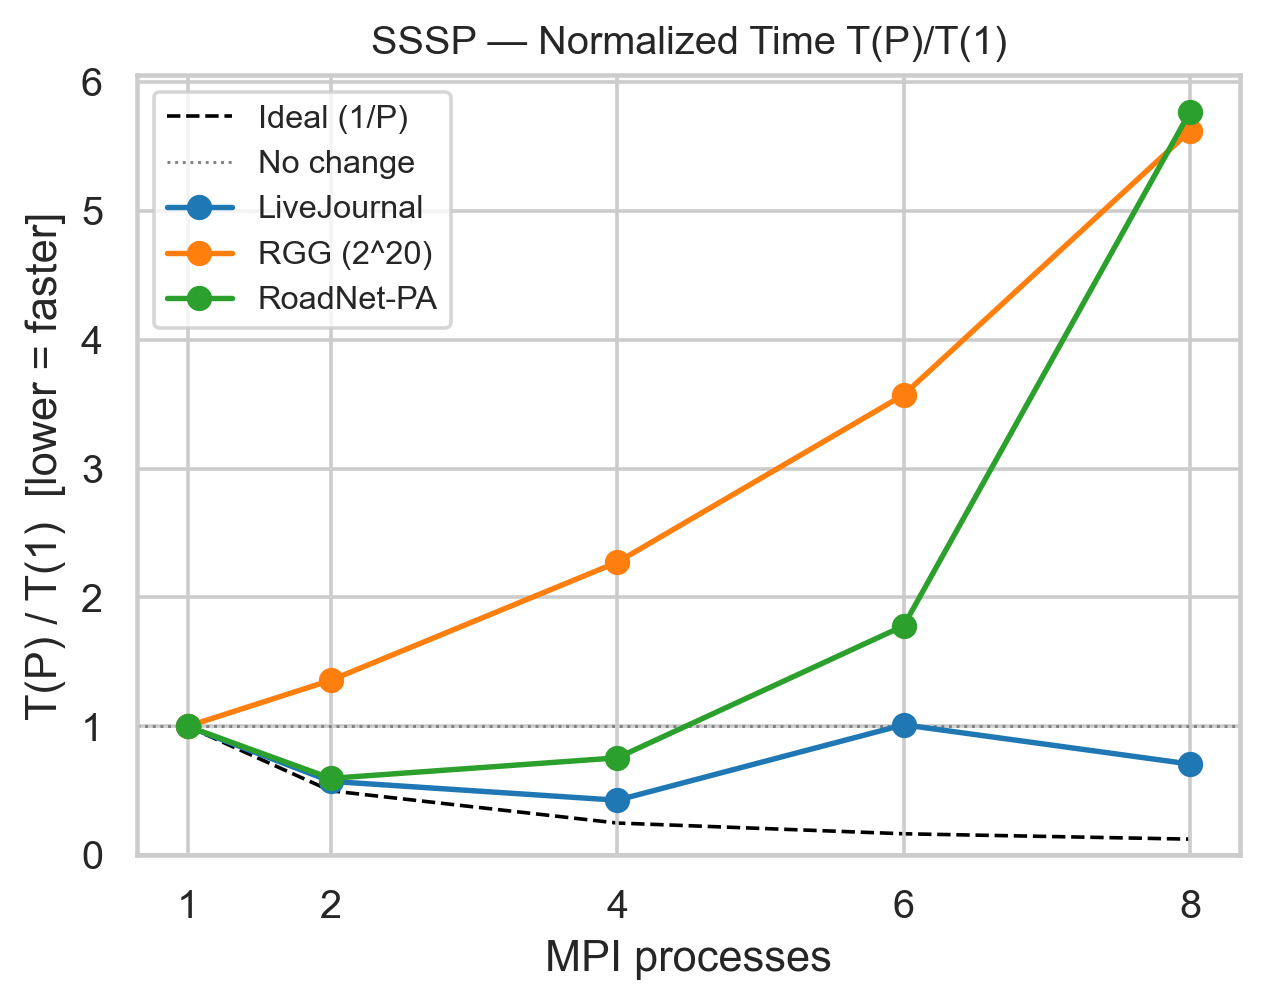
\includegraphics[width=0.5\textwidth]{../results/block2_t2/plots/speedup_sssp.png}
\end{frame}

% ──────────────────────────────────────────────────────────────────────────────
%  Поперечный анализ
% ──────────────────────────────────────────────────────────────────────────────


% ── Почему растут итерации ────────────────────────────────────────────────────
\begin{frame}
  \frametitle{Почему число итераций растёт с $P$?}

  \textbf{Причина --- staleness зеркал в BSP-модели:}
  \begin{enumerate}
    \item Мастер $v$ в итерации $k$ читает значение зеркала $\tilde{u}$
    \item $\tilde{u}$ содержит значение из \emph{предыдущего} раунда ---
          Gluon sync ещё не доставил обновление
    \item $v$ «не видит» улучшения и пропускает итерацию $k$
    \item На итерации $k{+}1$ зеркало обновлено --- $v$ наконец обновляется
    \item Больше процессов = больше зеркал = больше задержанных обновлений
  \end{enumerate}

\end{frame}

% ── Стоимость синхронизации ───────────────────────────────────────────────────
\begin{frame}
  \frametitle{От чего зависит стоимость синхронизации?}

  \[
    \mathrm{Cost}(\mathrm{sync}) \;\propto\;
    \underbrace{\mathrm{RF}(P)}_{\text{копий на вершину}}
    \;\times\;
    \underbrace{|V|}_{\text{вершин}}
    \;\times\;
    \underbrace{s}_{\text{байт/поле}}
    \;\times\;
    \underbrace{I(P)}_{\text{итераций}}
  \]

  \begin{itemize}
    \item \textbf{RF$(P)$}: для LJ $1.0 \to 1.62 \to 3.49$ при $P=1,2,8$
          --- в 3.5$\times$ больше данных на итерацию
    \item \textbf{$I(P)$}: PR/LJ $93 \to 410$ при $P=1\to8$
          --- в 4.4$\times$ больше раундов sync
    \item \textbf{Суммарно} трафик PR/LJ растёт
          $\approx 3.5\times4.4 \approx 15\times$ от $P{=}1$ к $P{=}8$
  \end{itemize}
\end{frame}

% ── Triangle counting ─────────────────────────────────────────────────────────
\begin{frame}
  \frametitle{Triangle Counting}

  \centering
  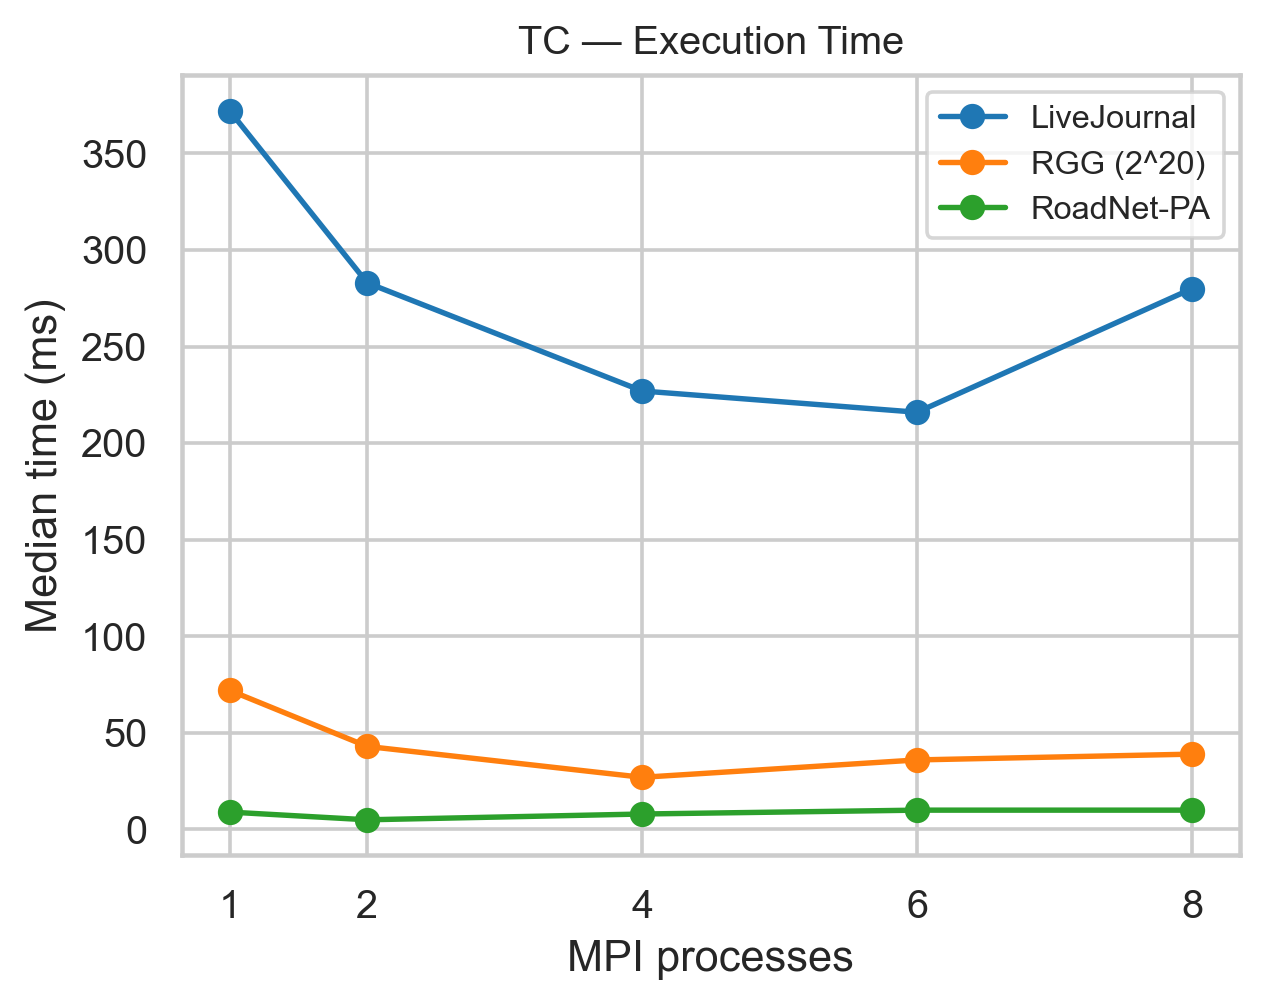
\includegraphics[width=0.5\textwidth]{../results/block2_t2/plots/time_tc.png}
\end{frame}

\begin{frame}
  \frametitle{Triangle Counting}

  \centering
  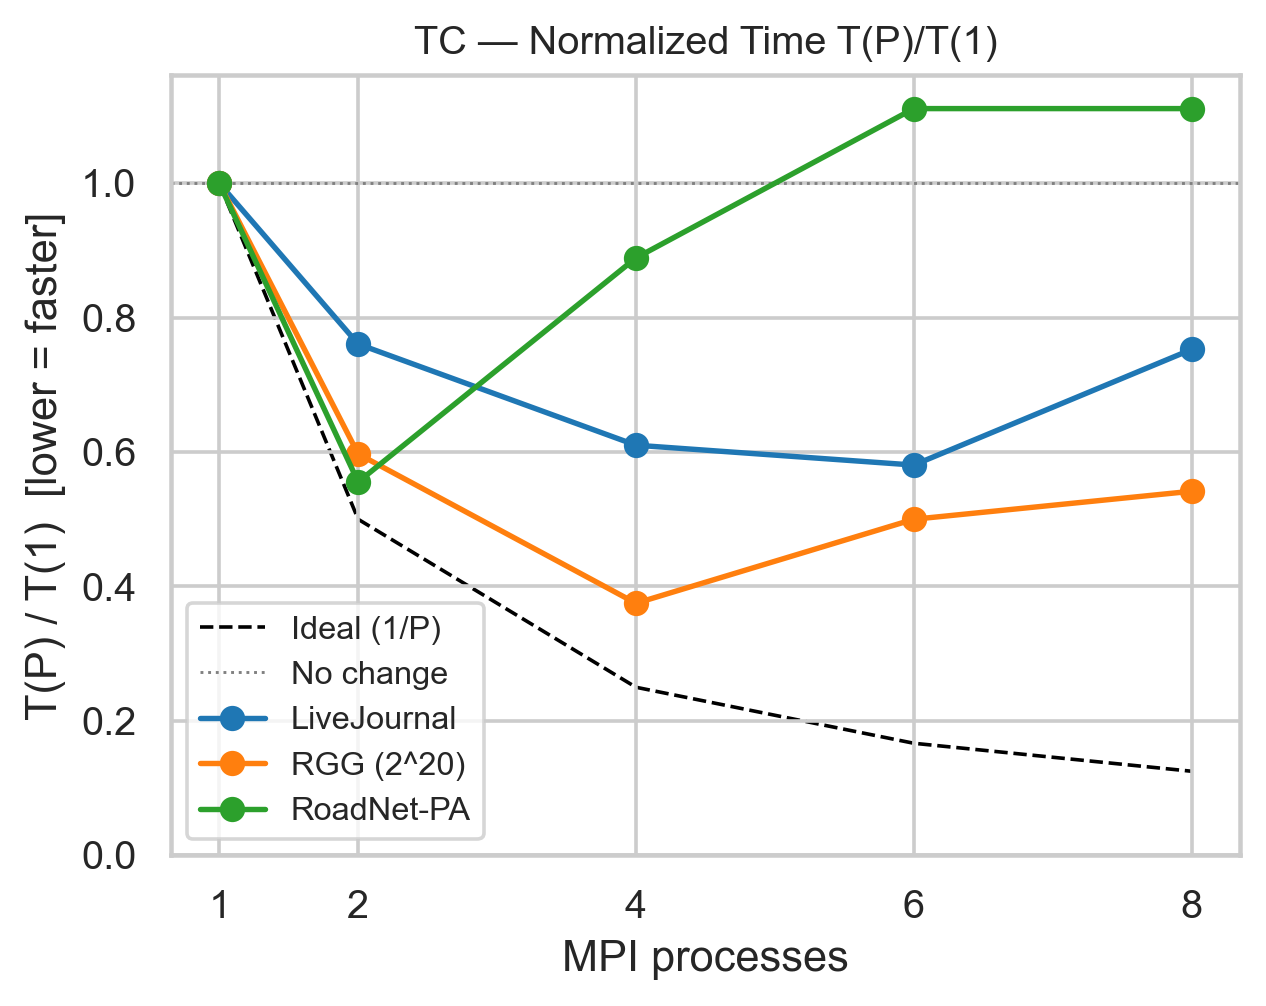
\includegraphics[width=0.5\textwidth]{../results/block2_t2/plots/speedup_tc.png}
\end{frame}

% ── Заключение ────────────────────────────────────────────────────────────────
\begin{frame}
  \frametitle{Заключение}

  {\small
  \begin{tabular}{p{5.6cm}p{5.8cm}}
    \hline
    \textbf{Вывод} & \textbf{Подтверждение} \\
    \hline
    BFS и SSSP на LJ ускоряются при $P{=}2$
    & $T(2)/T(1)=0.77$ и $0.79$ соответственно \\[4pt]
    LJ деградирует при $P{\ge}4$: RF растёт
    & RF\,$=3.49$ при $P{=}8$; $T(8)/T(1)>3.5$ \\[4pt]
    RGG --- вырожденный случай для BFS/SSSP
    & Итерации BFS: $495\to 2377$ ($P{=}1\to6$);\\
    & SSSP не сходится при $P{\ge}2$ \\[4pt]
    Итерации растут с $P$ (staleness зеркал)
    & PR/LJ: $93\to 410$; BFS/RGG: $495\to2377$ \\[4pt]
    Sync-cost $\propto$ RF$(P)\times I(P)$
    & LJ: оба множителя растут ($\times15$ итого) \\
    \hline
  \end{tabular}
  }

  \medskip
  {\small На реальном кластере (RTT $\sim$100\,мкс):
  накладные расходы на барьеры вырастут в 10--100 раз.
  Эффективны только конфигурации с малым диаметром и RF\,$\approx 1$.}
\end{frame}

% ── Приложение ────────────────────────────────────────────────────────────────
\appendix

\begin{frame}
  \frametitle{Справка: время выполнения при $P\times T=\mathrm{const}$}
  \centering
  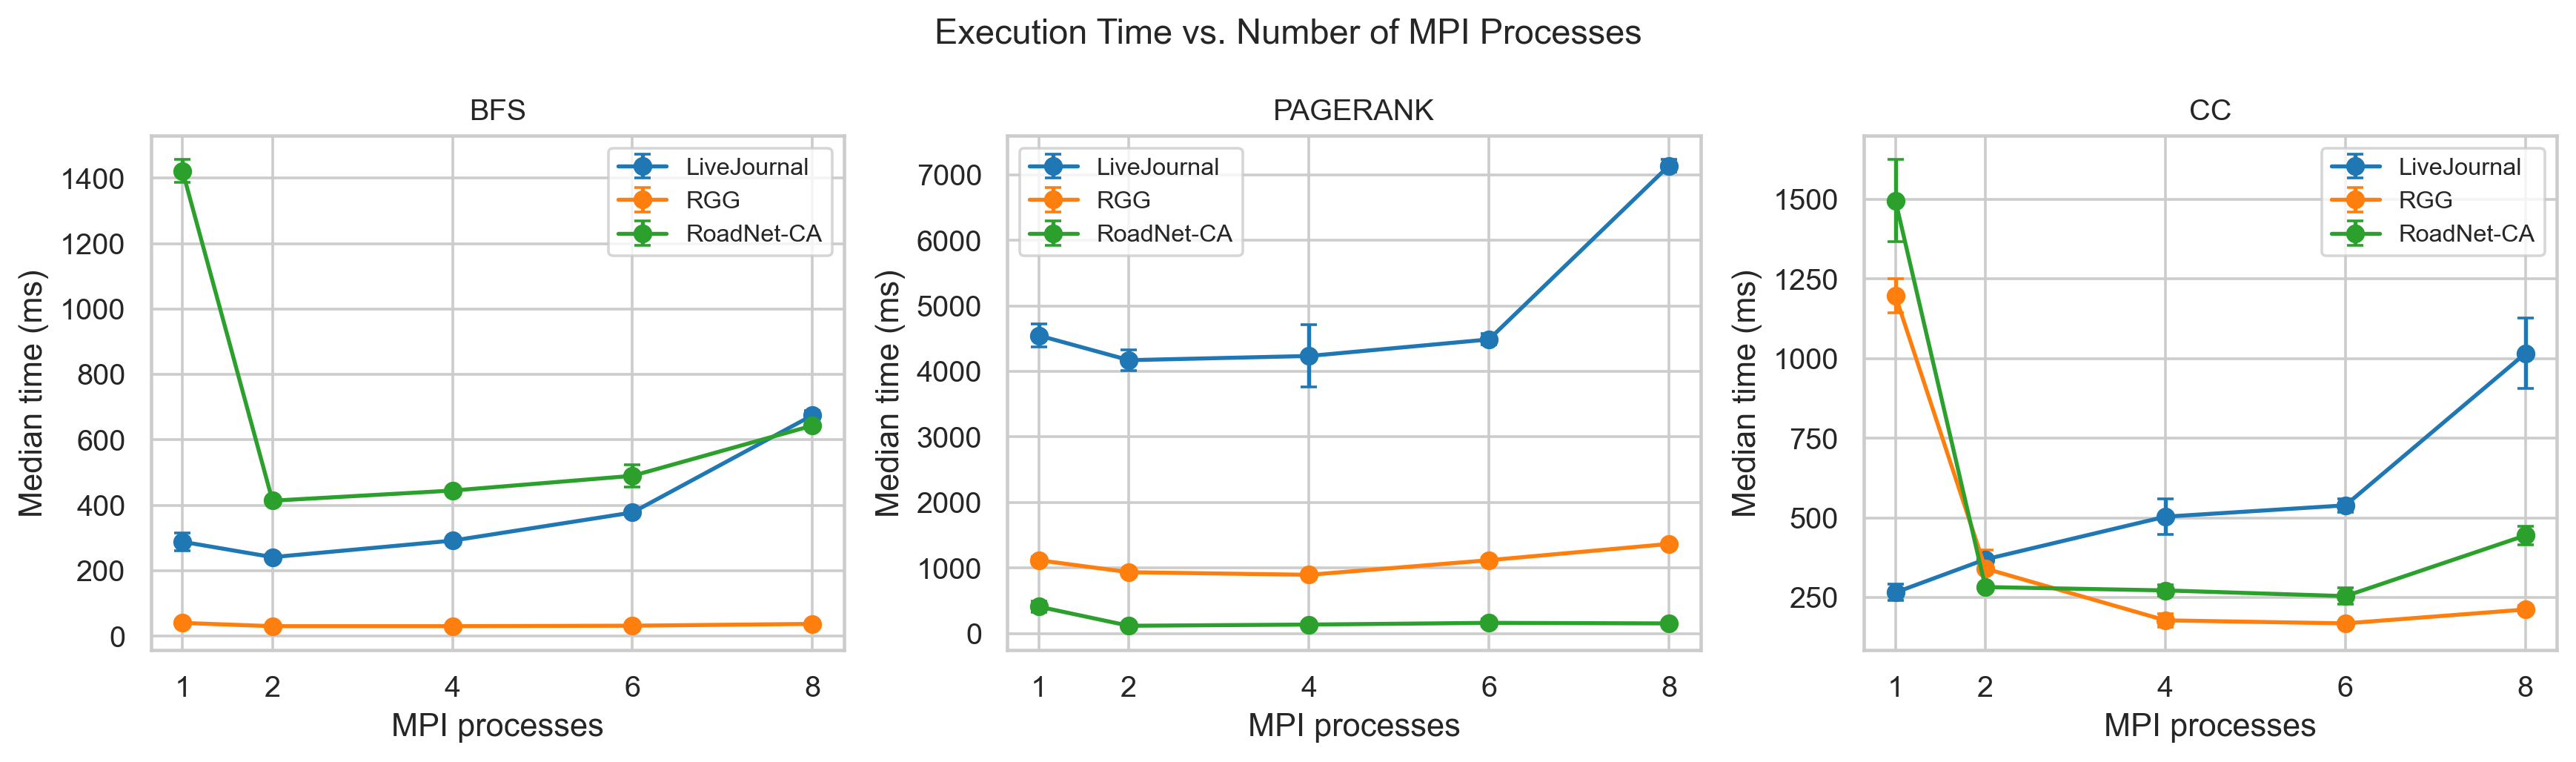
\includegraphics[width=1.0\textwidth]{../results/block2/plots/time_vs_hosts_ptconst.png}
\end{frame}

\begin{frame}
  \frametitle{Справка: нормализованное время при $P\times T=\mathrm{const}$}
  \centering
  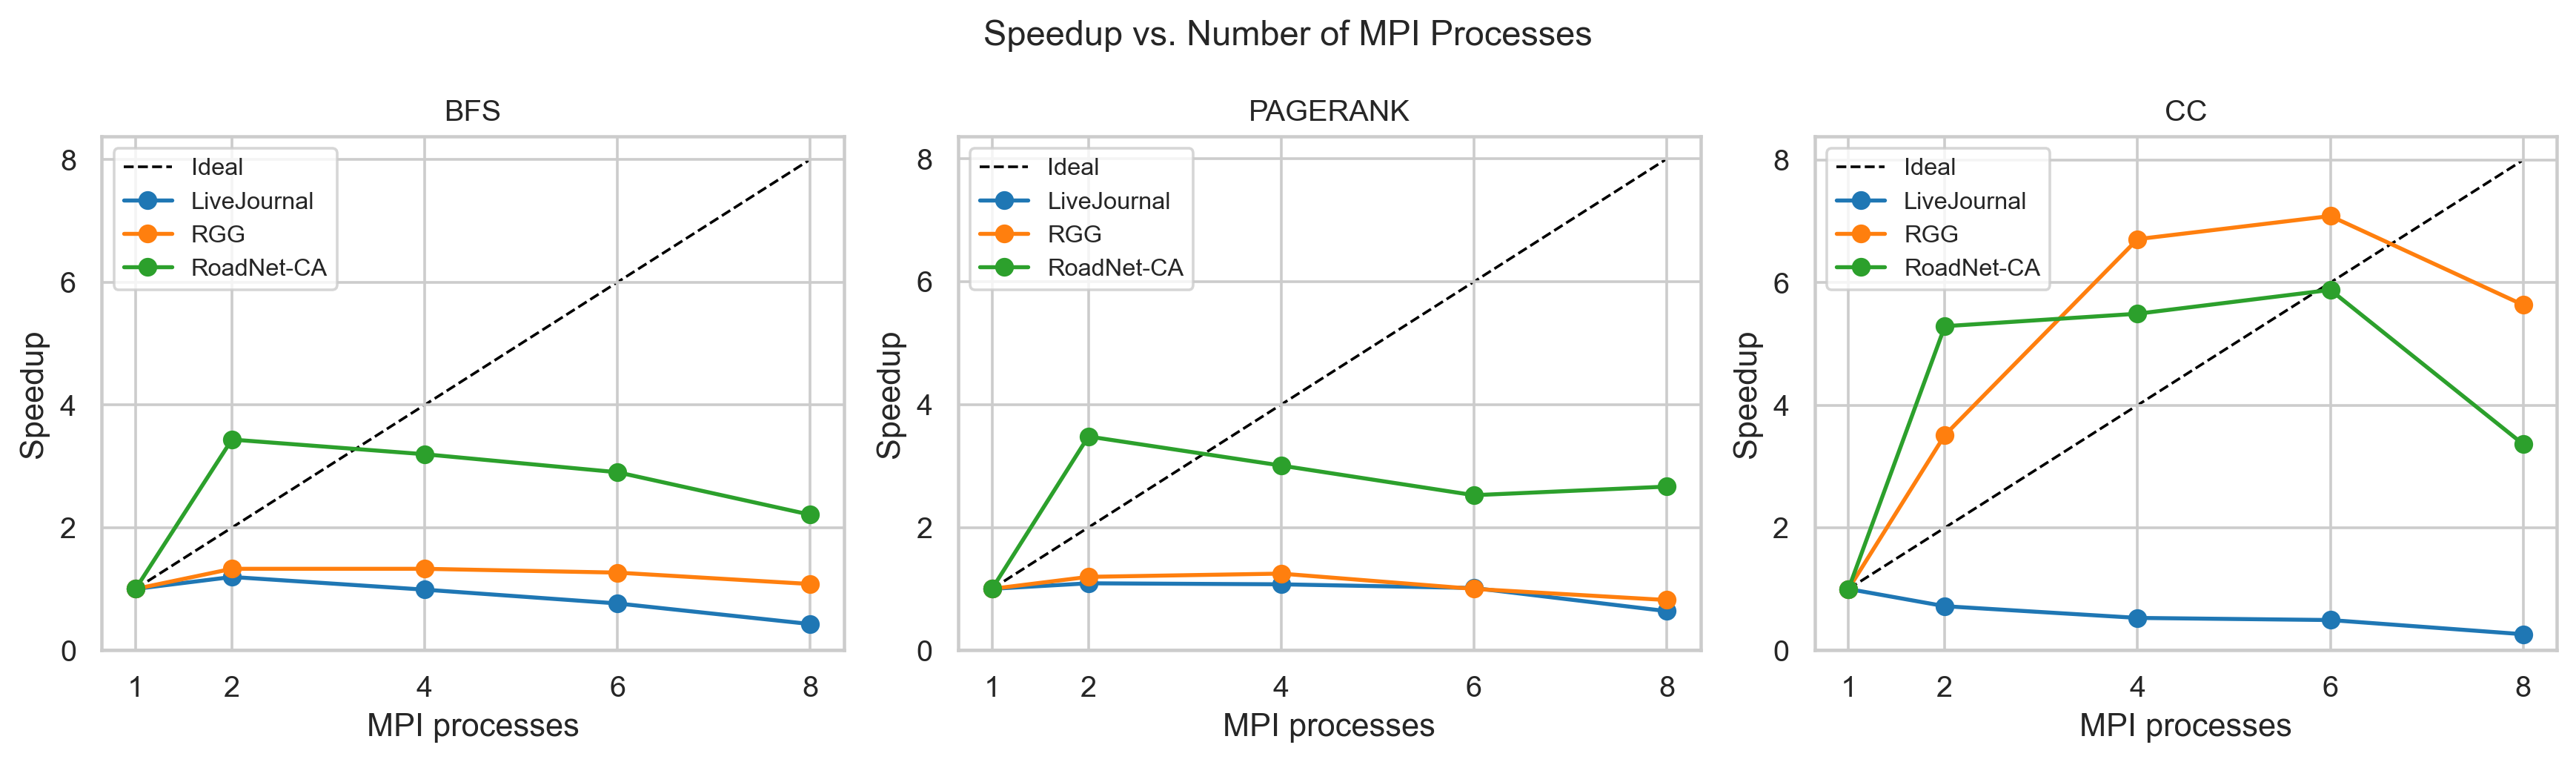
\includegraphics[width=1.0\textwidth]{../results/block2/plots/speedup_ptconst.png}
\end{frame}

\end{document}
